
\documentclass[10pt]{standalone}
\input{../tikzpic_packages.tex}
\begin{document}
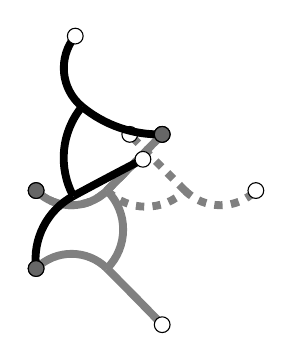
\begin{tikzpicture}
\tikzset{
    part/.style={line width = 1mm, color=gray},
    partD/.style={line width = 1mm, color=gray, dashed},
    partF/.style={line width = 1mm, color=black},
    foot/.style={fill=white},
    footfixed/.style={fill=\col},
    grid line/.style={white},
    start line/.style={help lines}}
\def\rfoot{.1}

\def\col{black!20}
\def\alpi{90.000000}
\def\beti{1.000000}
\def\gam{-90.000000}
\def\alpii{90.000000}
\def\betii{1.000000}
\def\gamh{-45.000000}

\def\eps{90.000000}
\def\ci{45.000000}
\def\cii{136.000000}
\def\ciii{315.000000}
\def\civ{224.000000}

\def\ri{0.636620}
\def\rii{57.295780}
\def\rg{-0.700282}
\def\riii{0.636620}
\def\riv{57.295780}

\path (0.000000, 2.000000)coordinate(F1);

\draw[part] (F1)arc(180+\ci:180+\ci+\alpi:\ri)coordinate(OM);
\draw[part] (OM)arc(180+\ci+\alpi:180+\ci+\alpi+\beti:\rii)coordinate(F2);
\draw[part] (OM)arc(90+\ci+\alpi:90+\ci+\alpi+\gam:\rg)coordinate(UM);
\draw[part] (UM)arc(\gam+\ci+\alpi:\gam+\ci+\alpi+\alpii:\riii)coordinate(F3);
\draw[part] (UM)arc(\gam+\ci+\alpi:\gam+\ci+\alpi-\betii:\riv)coordinate(F4);

\draw[footfixed] (0.000000, 2.000000)circle(\rfoot);
\draw[foot] (1.601217, 2.713241)circle(\rfoot);
\draw[foot] (0.000000, 1.009652)circle(\rfoot);
\draw[foot] (1.601217, 0.296411)circle(\rfoot);








\def\col{black!60}
\def\beti{1.000000}
\def\alpi{90.000000}
\def\gam{90.000000}
\def\betii{1.000000}
\def\alpii{90.000000}
\def\gamh{45.000000}

\def\eps{180}
\def\cii{44.000031}
\def\ci{135.000031-90}
\def\civ{136.000031}
\def\ciii{45.000031}

\def\rii{57.295779}
\def\ri{0.636620}
\def\rg{0.700282}
\def\riv{57.295780}
\def\riii{0.636620}

\path (0.000000, 2.000000)coordinate(F1);

\draw[partD] (F1)arc(180+\ci:180+\ci+\alpi:\ri)coordinate(OM);
\draw[partD] (OM)arc(180+\ci+\alpi:180+\ci+\alpi+\beti:\rii)coordinate(F2);
\draw[partD] (OM)arc(90+\ci+\alpi:90+\ci+\alpi+\gam:\rg)coordinate(UM);
\draw[partD] (UM)arc(\gam+\ci+\alpi:\gam+\ci+\alpi+\alpii:\riii)coordinate(F3);
\draw[partD] (UM)arc(\gam+\ci+\alpi:\gam+\ci+\alpi-\betii:\riv)coordinate(F4);

\draw[footfixed] (0.000000, 2.000000)circle(\rfoot);
\draw[footfixed] (1.601217, 2+2-1.286759)circle(\rfoot);
\draw[foot] (1.601217+0.411453+.8, 2.000000) (F3)circle(\rfoot);
\draw[foot] (1.601217-1.189763+.8, 4-1.286758) (F4)circle(\rfoot);








\def\col{black!60}
\def\alpi{90.000000}
\def\beti{40.840020}
\def\gam{67.837900}
\def\alpii{68.989560}
\def\betii{1.000000}
\def\gamh{33.918950}

\def\eps{84.414291}
\def\ci{320.495341}
\def\cii{91.335361}
\def\ciii{7.322802}
\def\civ{297.333241}

\def\ri{0.636594}
\def\rii{1.543225}
\def\rg{1.021964}
\def\riii{0.913549}
\def\riv{57.293496}

\path (0.497329, 3.961480)coordinate(F1);

\draw[partF] (F1)arc(180+\ci:180+\ci+\alpi:\ri)coordinate(OM);
\draw[partF] (OM)arc(180+\ci+\alpi:180+\ci+\alpi+\beti:\rii)coordinate(F2);
\draw[partF] (OM)arc(90+\ci+\alpi:90+\ci+\alpi+\gam:\rg)coordinate(UM);
\draw[partF] (UM)arc(\gam+\ci+\alpi:\gam+\ci+\alpi+\alpii:\riii)coordinate(F3);
\draw[partF] (UM)arc(\gam+\ci+\alpi:\gam+\ci+\alpi-\betii:\riv)coordinate(F4);

\draw[footfixed] (1.601217, 2.713241)circle(\rfoot);
\draw[footfixed] (0.000000, 1.009652)circle(\rfoot);
\draw[foot] (0.497329, 3.961480)circle(\rfoot);
\draw[foot] (1.356792, 2.397076)circle(\rfoot);

   
\end{tikzpicture}
\end{document}
